\section{Detector infrastructure}
\label{ch:dp-tc-infrastructure}

The detector infrastructure for the \dword{dpmod} comprises the equipment used by several groups and consortia to install and operate the detector.
It includes the electronics racks on top of the mezzanine on the cryostat roof and the related networking, electrical and cooling power, cable trays, cryostat penetrations and flanges, detector ground isolation transformers, and monitors.
Inside the cryostat, the detector infrastructure includes the gas and liquid argon distribution manifolds, the cryostat false floor to protect the corrugated membrane and allow safe circulation of material and people inside the cryostat, movable scaffold and man lifts for activities at height, and the ventilation and air circulation and filtration.
A cleanroom equipped with  \coldbox{}es for the functional tests of the \dwords{crp} is also present in front of the \dword{tco}.
This cleanroom and the cryostat itself are the places where some detector components are manipulated and assembled before installation.

\subsection{Cryostat Roof}
The roof of the \dword{dpmod} cryostat is going to be very dense with equipment, more so than the \dword{spmod}.
Ideally all the roof surface that is not equipped with feedthroughs and racks should be walkable.
For this reason, at the same height of the cryostat I-beams, a floor capable of standing at least 250~kg/m$^2$ is installed.
The floor is not meant to move heavy material around the roof.
The material of the floor must comply with the safety rules in force.
Plywood painted with flame retardant agents may be a cost-effective and adequate option; that must be confirmed with \dword{esh}.
No pipes, tubing, or cable trays along the length or the width of the cryostat should be installed above the false floor, in order to minimize the risk of accidents to personel and material due to tripping.
The floor must segmented in sections that are easily opened by one person to allow easily access to the equipment underneath.
The most convenient passage to cross the entire length of the cryostat will be under the detector rack mezzanine.
Lighting under the cryogenics and the detector mezzanines will be available.
During cryostat construction, welding of the pipes and flanges, and installation of the cable trays, the false floor must be installed only in the zones dedicated to the passage, considering that the co-activity during these periods is expected to be high and each worker should have enough space to safely work and move.

A drawing of the full cryostat roof with its penetrations is shown in Figure~\ref{fig:DP-roof-penetration}.
A zoom of the same image of a corner on the opposite side of the \dword{tco} is shown in Figure~\ref{fig:DP-roof-penetration-zoom}.
The same figure shows also the \threed model of the roof with equipment on the \dword{crp} support and \dword{sgft} penetrations.
This image highlights the high density of the equipment on the \dword{dpmod} roof, even more important considering that each of these flanges will be reached by several cables.

\begin{dunefigure}[Drawing of \dshort{dpmod} roof]{fig:DP-roof-penetration}
{Drawing of the cryostat roof with its penetrations.}
\includegraphics[width=0.9\textwidth]{DP-roof-penetration.png}
\end{dunefigure}

\begin{dunefigure}[Zoom of the \dshort{dpmod} roof]{fig:DP-roof-penetration-zoom}
{Zoom of the \dword{dpmod} roof drawing (left) and 3D model of the same portion of the roof with the \dword{sgft} and \dword{crp} suspension chimneys instrumented.}
\includegraphics[width=0.45\textwidth]{DP-roof-penetration-zoom.png}
\includegraphics[width=0.45\textwidth]{DP-roof-penetration-3D.png}
\end{dunefigure}

The role of the roof penetrations is to connect the ultra-pure argon volume to the atmosphere through the roof insulation, while minimizing the heat input.
All the penetrations are on the roof of the cryostat except the ones for the liquid argon re-circulation that are at the bottom of the \dword{tco} wall.
The sketch of a typical roof penetration cross-section is shown in Figure~\ref{fig:penetration-cross-section-sketch}.
\begin{dunefigure}[Sketch of a typical roof penetration]{fig:penetration-cross-section-sketch}
{Sketch of a typical roof penetration.}
\includegraphics[width=0.9\textwidth]{penetration-cross-section-sketch.png}
\end{dunefigure}
The thermal insulation is installed around a vertical stainless steel pipe that is mechanically connected to the walls of the warm structure.
The corrugated membrane is welded vacuum tight to the pipes.
The excess pipe inside the cryostat volume may be used to weld a mechanical support, for instance to attach cable trays.

On the atmospheric side a \dword{uhv} CF flange is welded vacuum tight to the pipe.
Except for the four access ports, all the flanges on the chimneys follow the \dword{uhv} CF flange standard ISO 3669:2017.
The leak rate of this widespread standard vacuum connections is lower than $10^{-9}$~mbar$\times$L/s.
The feedthroughs and the mating flanges are expected to be compatible with this level of leaks.
All the penetrations, the flanges, and the feedthroughs will be leak tested in situ after the final installation with helium sniffing techniques sensitive to local leaks of $10^{-6}$~mbar$\times$L/s.
More sensitive techniques (like vacuum bags) may be applied to selected feedthroughs and penetrations if required.

The welded flanges on the roof may need to be supported in case they must sustain significant load, as for example in the case of the penetrations for the \dword{crp} and field cage supports.
These flanges carry out the role of interface between the cryostat and the feedthroughs.
The scope of the detector infrastructure ends at the flange.
Copper gaskets, bolts, and nuts are in the scope of the mating flange or feedthrough.
The holes for the bolts on the cryostat flanges are not threaded.
Special nuts may be needed if the support/reinforcement structure underneath the flange makes the tightening of the bolts too difficult.

In order to allow an effective air purge, each penetration will be outfitted with an exhaust. Each penetration is therefore equipped with 12~mm outer diameter pipes welded on the tube penetration.
This pipe is then connected to the main purge manifold by means of stainless steel flexible tubes.
The exhaust should be positioned high enough in order to minimize air pockets.
If the feedthrough extends significantly in the vertical direction form the roof flange, it is preferred that the exhaust is placed on the feedthrough flange itself.
The connection to the manifold is done in the same way with flexible tubing, while the exhaust welded on the penetration tube is vacuum sealed with the proper tube plug.

During the cryostat purging, the gas from the roof penetrations is exhausted through the dedicated pipes provided by the cryogenics system.
It is sampled with oxygen, nitrogen, and moisture analysers in order to define the argon gas purity.
This measurement determines the \cooldown and  filling process starts.
During operation, instead, the majority of the argon from the roof penetration is purified and re-condensed.
A fraction of it is analysed in order to study the internal sources of pollution (for instance cables) and to reveal the appearance of leaks.

On/off valves pneumatically controlled by the cryogenics control system are installed between the exhaust manifold and the penetrations.
A single valve may collect the flow from multiple neighboring penetrations.
The number of valves and the pattern of interconnections will be defined later also taking into account budget constraints.
The role of these valves is twofold: (1) They are used to isolate the gas flow from few selected penetration in order to study the location of the internal pollution sources. (2) They are used during the leak tests of the feedthroughs to feed helium gas in the chosen penetrations.

There are several kinds of penetrations that serves different needs.
Table~\ref{tab:penetrations} summarizes all of them.
\begin{dunetable}[Types of penetrations through the roof]
{cccccc}
{tab:penetrations}
{Types of penetrations through the roof.}
Type & Number & CF & Pipe ID (mm) & Ext. Sup. & Int. Sup.\\
\toprowrule \dword{crp} sup. & 240 & CF100 & 100 & yes & no\\
\colhline Field cage sup. & 24 & CF150 & 150 & yes & no\\
\colhline \dword{crp} inst. & 42 & CF250 & 250 & no & yes\\
\colhline Tank inst. & 20 & CF250 & 250 & no & yes\\
\colhline \dword{sgft} & 240 & CF275 & 267 & yes & no\\
\colhline VHV & 1 & CF250 & 250 & no & yes\\
\colhline Manhole & 4 & custom & 700 & no & no\\
\colhline Cryo & 39 & various & various & various & various\\
\end{dunetable}
\begin{comment}
\begin{dunetable}[Types of penetrations through the roof]
{ccccccc}
{tab:penetrations}
{Types of penetrations through the roof.}
Type & Number & CF & Pipe OD (mm) & Pipe ID (mm) & Ext. Sup. & Int. Sup.\\
\toprowrule \dword{crp} sup. & 240 & CF100 & 104 & 100 & yes & no\\
\colhline Field cage sup. & 24 & CF150 & 154 & 150 & yes & no\\
\colhline \dword{crp} inst. & 42 & CF250 & 254 & 250 & no & yes\\
\colhline Tank inst. & 20 & CF250 & 254 & 250 & no & yes\\
\colhline \dword{sgft} & 240 & CF275 & 273.2 & 267 & yes & no\\
\colhline VHV & 1 & CF250 & 254 & 250 & no & yes\\
\colhline Manhole & 4 & custom & 706 & 700 & no & no\\
\colhline Cryo & 39 & several & several & several & several & several\\
\end{dunetable}
\end{comment}
Interface documents stating the requirements and the constraints on the internal diameter of the penetration tube, on its linearity and verticality, and on the horizontality and orientation of the welded flanges will be agreed with the \dword{dune} consortia and the cryogenics.
The experience gained with \dword{pddp} showed that the most critical penetrations in this respect are the ones of the \dword{sgft}.
For this reasons, the internal dimension of the \dword{sgft} penetration pipes was increased to 267~mm.
The pipes of the penetration for the \dword{crp} suspensions are also increase to 100~mm internal diameter.

Table~\ref{tab:load-penetration} summarizes the penetration flanges subjected to significant mechanical loads for different conditions.
These require external supports.
\begin{dunetable}[Load for mechanical support penetrations]
{cccc}
{tab:load-penetration}
{Load for mechanical support penetrations.}
Type & Number & Empty (kg) & Full (kg) \\
\toprowrule \dword{crp} sup. & 240 & 150 & 150\\
\colhline Field cage sup. & 24 & 1100 & 700 \\
\colhline \dword{sgft} & 240 & 120 & 120 \\
\end{dunetable}

The support system for the \dwords{crp} is described in the \dword{crp} chapter of this \dwords{tdr}.
Each \dword{crp} is suspended at three points connected to the external \dword{crp} supports through the chimneys.
During \dword{crp} installation this system allows attachment of the \dwords{crp} at the level of the cryostat internal floor followed by lifting them up to their final position.
In this condition, the system allows manual horizontal adjustment of $\pm 26$~mm and electrically controlled vertical adjustment of $\pm 40$~mm.
The vertical movement is used to adjust the horizontality of the height of the \dwords{crp} with respect to the \dword{lar} level.
The horizontal movement allows minimization of the uninstrumented surface arising from the thermal shrinkage of the \dwords{crp}.
The cryostat structural I-beams are spaced every 1.6~m, while the \dword{crp} size is $3\times3$~m$^2$.
In order to avoid interference between the I-beams and the \dword{crp} support system, the position hanging points is not always the same for all the \dwords{crp}.
There are two different triangular patterns and the \dword{crp} structure copes with boths.
The \dword{crp} will have different hancoring points to meet the different positions of the penetrations.

The heaviest load that this system must withstand is during the lifting of the \dwords{crp} and the opening of the protection box.
The estimated load for each penetration in this condition is 240~kg.
Square steel tubes solidly welded to the cryostat main I-beams will support the weight.
Analogous reinforcement are expected for the field cage support penetrations.
These reinforcement are installed at the same time when the flanges will be welded on the penetration pipes.
The detailed design of these elements is not defined yet.
The equivalent implementation of the supports in \dword{pddp} is shown in Figure~\ref{fig:mechanical-supports}.
\begin{dunefigure}[Mechanical support of the \dshort{crp} and \dshort{fc} support penetrations in \dshort{pddp}]{fig:mechanical-supports}
{Photos of the mechanical support of the \dword{crp} (left) and field cage (right) support penetrations implemented in \dword{pddp}.}
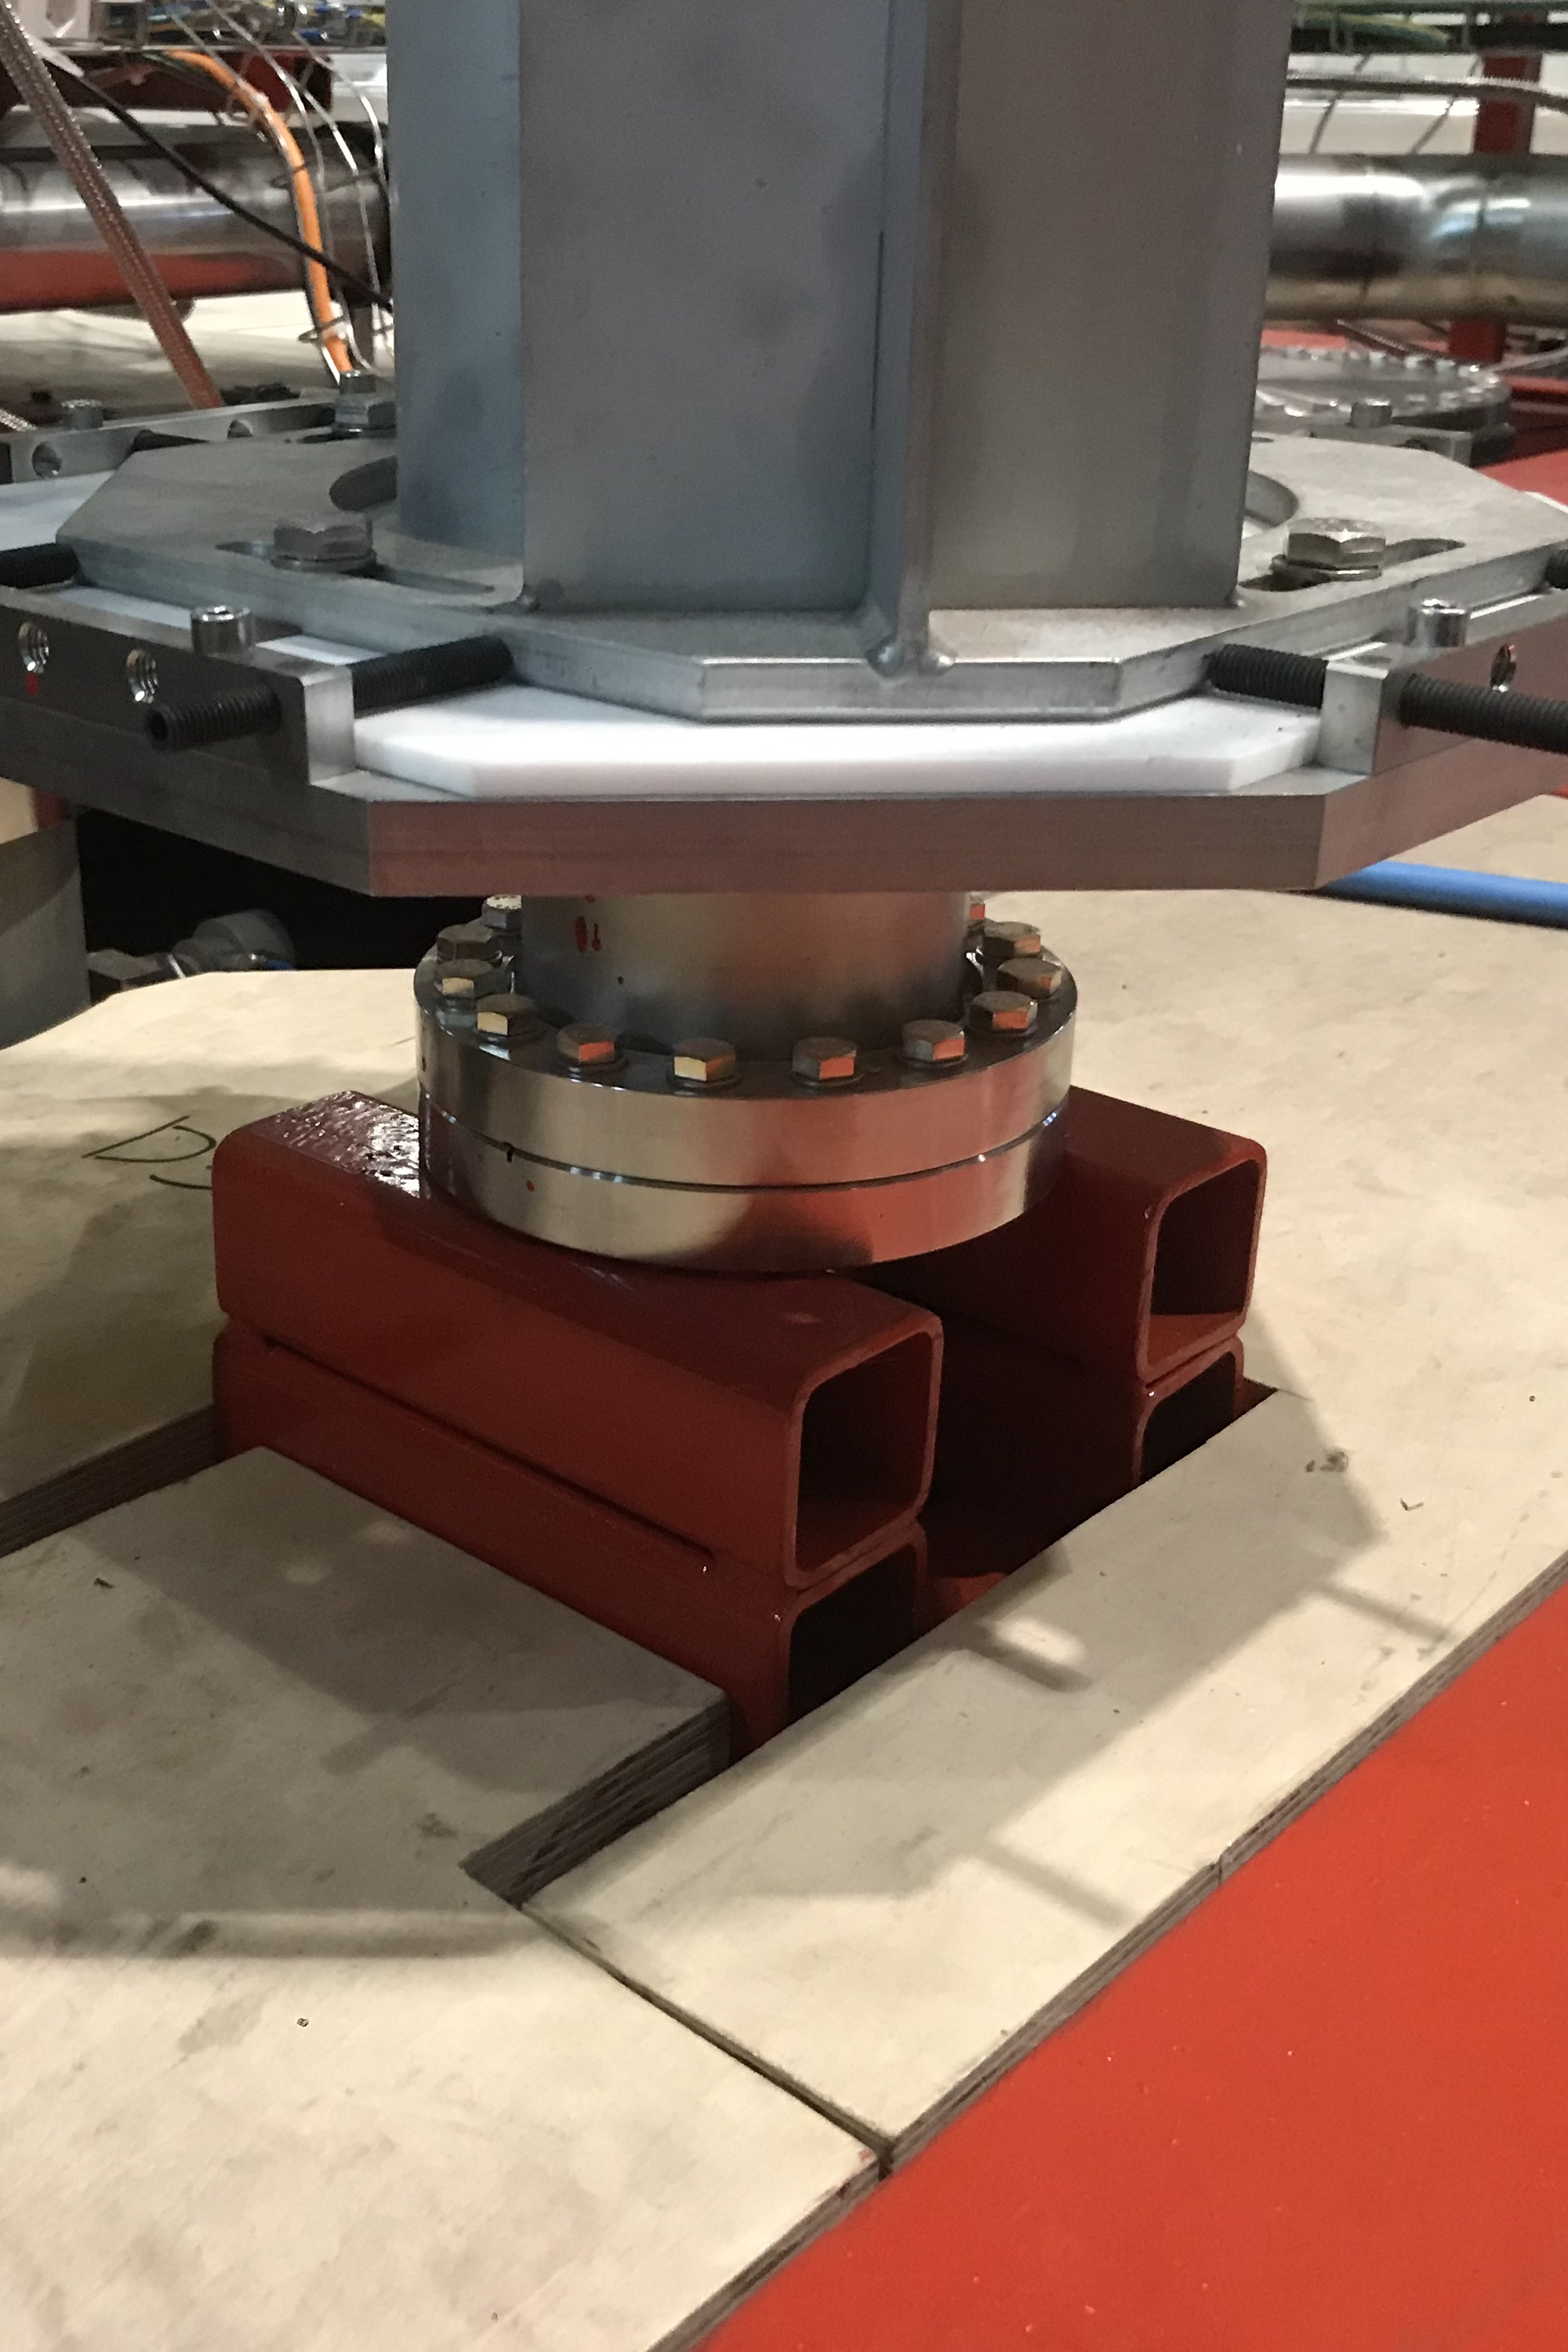
\includegraphics[width=0.45\textwidth]{crpSupport.jpg}
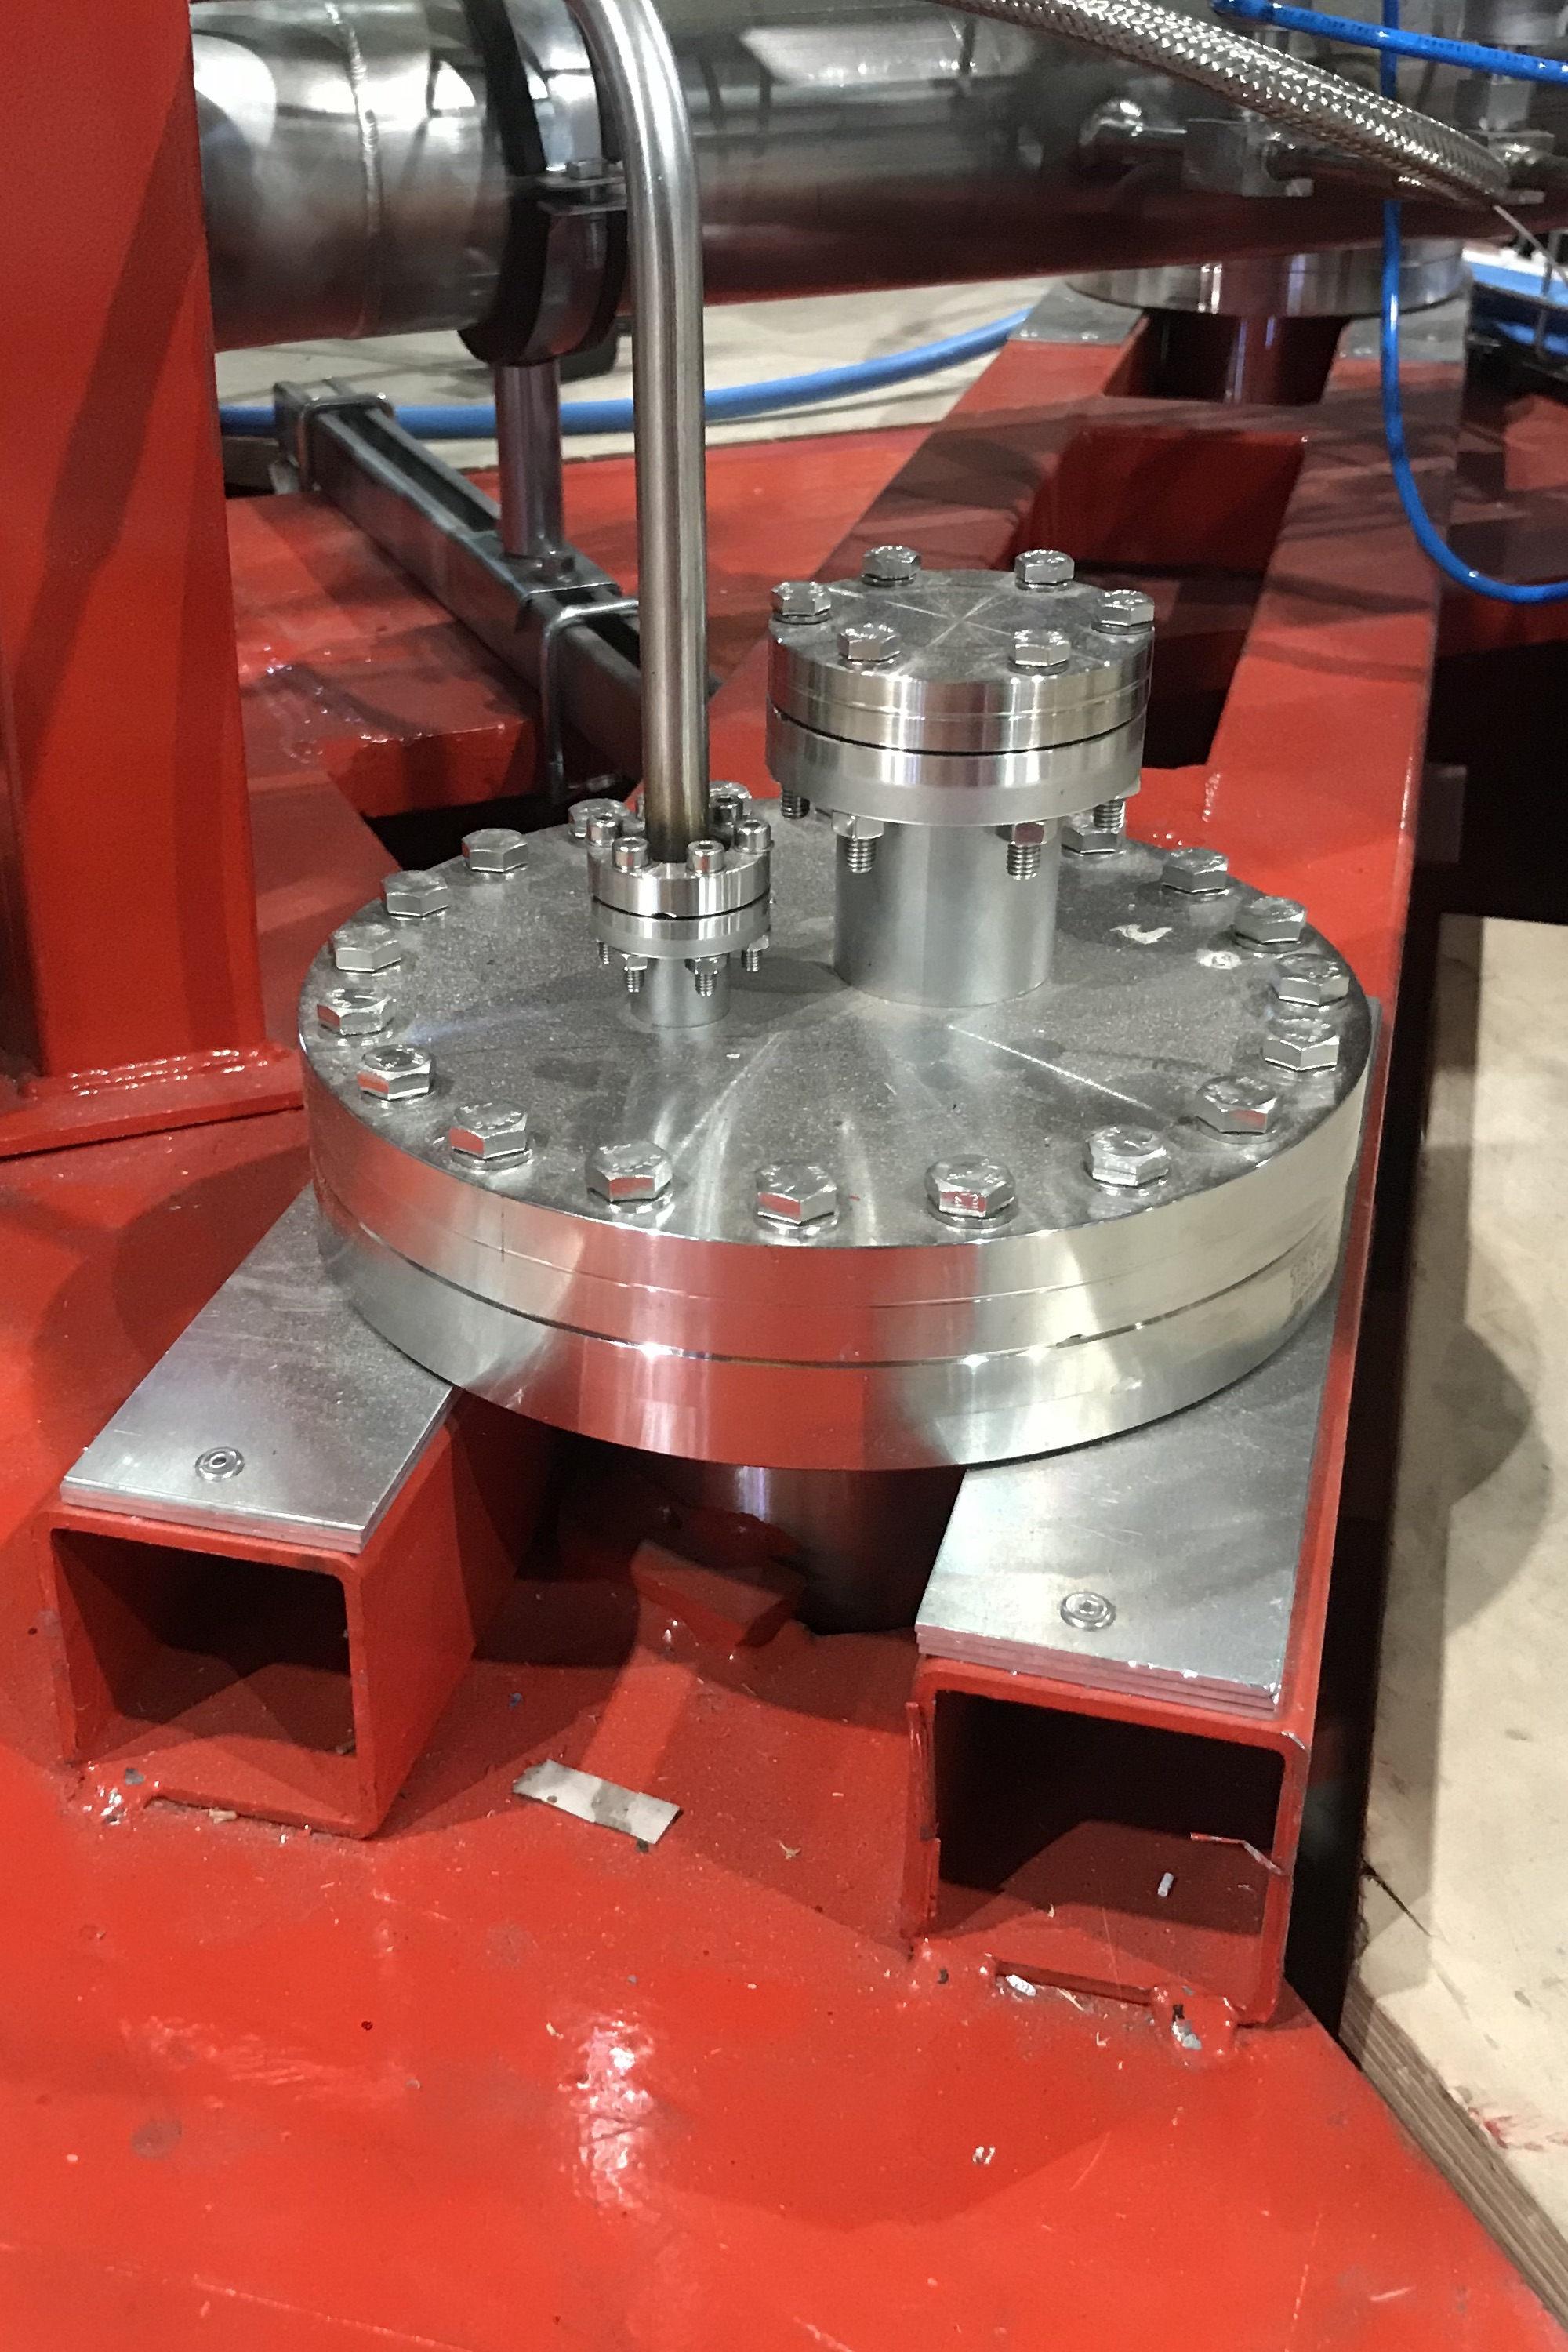
\includegraphics[width=0.45\textwidth]{fieldCageSupport.jpg}
\end{dunefigure}

All the service cables for the operation of the \dwords{crp} enters into the cryostat from what are called \dword{crp} instrumentation penetrations.
The cables passing through these penetrations are the HV for the \dword{lem} and the extraction grid, the coaxial cables for the distance meters and the level meters, the ground shielded cables for the temperature sensors, and the multi twisted pairs for the anode pulsing.
Each penetration serves two CRPs, and is positioned approximately between two adjacent \dwords{crp}.
The couple of \dwords{crp} are chosen to guarantee that during the installation sequence (from left to right in Figure~\ref{fig:DP-roof-penetration}) the penetration is always accessible by means of an elevating platform or a movable scaffold once the \dwords{crp} are in final position.
Due to the presence of the cryostat I-beams, the position of these penetrations is not symmetric with respect to the length of the cryostat.
The cabling from one of the two \dwords{crp} will be more difficult.
Internal cable trays/cable support system welded to the excess penetration tube inside of the cryostat will be used to lay the cables and guide them through the penetration releasing the mechanical stress on the connections due to the cable weight.

The field cage walls, and consequently the cathode, are attached to the roof through the field cage support penetrations.
Ten of these penetrations run along each of the long walls and two along each of the short walls.
These penetrations are used during installation: a mechanisms of pulleys the field cage is lifted from the floor inside the cryostat and lifted up to final position while actually assembling the wall.
From the same penetration the field cage will be finally hanging.
Due to the geometry of the detector and the size of the instrumented surface these penetration are unavoidably very close to the cryostat I-beam.
Along the short walls the four penetration are actually going through the I-beams, that must be therefore specially modified and consequently reinforced.
The size of the internal diameter of these penetration is large enough to allow thermal shrinkage of the field cage and cathode.

The so-called tank instrumentation penetrations are twenty openings in the roof along the cryostat long direction on both the sides.
They are meant to pass cables an instrumentation for the power and signal of the photon detectors, the optical fibers for their calibration, cable and fibers for level meters, cryogenic cameras and lighting, temperature sensors and profilers, purity monitors, and in general all the cryogenics instrumentation devices installed inside of the cryostat.
No cable trays can be connected directly to the corrugated membrane.
The cables trays can run along the internal edges of the membrane where threaded rods are welded to allow the installation of cable supports.
Dedicated cable supports and stress release devices are welded from the portion of the penetration pipe exceeding the corrugated membrane to guide the cable through penetration.
In addition, cable supports can be connected to the cryogenic pipes of the cooling sprayers to guide cables and optical fibers from the top to the bottom of the cryostat (see Figure~\ref{fig:internal-cryogenics}).

The unique \dword{hv} feedthrough penetration is located inside the surface delimited by the field cage, in correspondance of the active volume of the detector.
This design decision is due to the fact that the space between the field cage and the corrugated membrane is not sufficient to guarantee that 600~kV can be safely applied at the cathode, without the risk of electrical breakdown to ground.
The penetration is located in a corner of the \dword{tpc} underneath the detector rack mezzanine on the \dword{tco} wall.
The length of the feedthrough allows it to be inserted in the penetration when the mezzanine is in place.
The connection between the feedthrough and the cathode must go through a \dword{crp} that must therefore be special: 1~m$^2$ will not be equipped with anodes, \dwords{lem} and extraction grid.
This \dword{crp} must be installed and cabled before the connection from the \dword{hv} feedthrough and the cathode is established.

The \dword{sgft} were developed first for the 3x1x1 detector at \dword{cern} and then applied to the \dword{pddp} with a slightly different design.
Their role is to allow the electronics to be near the anode electrodes (minimize the cable lengths) and in cold (reduce the intrinsic noise of the electronics) while still having the possibility to extract the electronics without compromising the liquid argon purity.
The drawing of the \dword{sgft} used in \dword{pddp} is shown in Figure~\ref{fig:sgft-drawing}.
\begin{dunefigure}[\dshort{sgft} drawing]{fig:sgft-drawing}
{Drawing of the \dword{sgft} used in \dword{pddp}.}
\includegraphics[width=0.9\textwidth]{sgft-drawing.png}
\end{dunefigure}

The \dword{sgft} are tubes through the cryostat roof insulation.
Their inner volume is isolated form the argon and from the atmosphere.
The electronics is installed inside the tube at a level few cm below the corrugated membrane of the cryostat roof.
At the cold side of the \dword{sgft}, a flange hosts electrical connectors that connect the cables to the anode at one side and the cold electronics at the other (see Figure~\ref{fig:sgft-picture}).
A system of guiding rails along the length of the \dword{sgft} ensures that the electronics can be correctly plugged into the cold flange.
\begin{dunefigure}[\dshort{sgft} picture]{fig:sgft-picture}
{Image of the flange and the tube of the \dword{sgft} used in \dword{pddp} prior assembly.}
\includegraphics[width=.5\textwidth]{sgft-picture.jpg}
\end{dunefigure}
This flange is crucial because at cold it isolates the ultra-pure argon.
The \dword{sgft} volume is filled with nitrogen or argon to avoid moisture condensation on the electronics.
The temperature at the bottom of the \dword{sgft} is not low enough to allow the condensation of argon.
Having argon at 1~bar as the atmosphere inside the \dwords{sgft} would reduce the possible \dword{lar} contamination consequent to the development of a leak in the cold flange.
Each \dword{sgft} before installation must be electrically tested and helium leak must be proven to be better than $10^{-8}$~mbar$\times$L/s at room temperature.
At least the cold flanges must be leak tested at cryogenic conditions too.

%DESCRIPTION OF THE LAYOUT OF THE CABLE TRAYS. NOT YET FULLY DEFINED.

%DESCRIPTION OF THE LAYOUT OF THE ELECTRONICS RACKS. NOT YET FULY DEFINED.

%BRIEF DESCRIPTION OF THE PURGE PIPES. SCOPE OF THE CRYOGENICS.

\subsection{Cryostat Interior}
The internal cryogenics comprises manifold of pipes to ensure the proper detector purge, cool-down, filling and re-circulation of \dword{lar}.
A 3D view of the inside of the \dword{dpmod} with the cryogenic pipes is shown in Figure~\ref{fig:internal-cryogenics}
All pipes enter the cryostat from the cryo penetrations on the roof.
The \dword{gar} distribution system consists of a set of pipes installed on the cryostat floor (shown in red in Figure~\ref{fig:internal-cryogenics}).
These pipes are used only prior to filling to remove the air in the cryostat.
They have either a longitudinal slit or calibrated holes to distribute \dword{gar} uniformly along the length of the cryostat.
The piston purge effect was successfully tested in \dword{pdsp} and  \dword{pddp}.
In order to efficiently extract the air, turbulence must be avoided while purging with warm \dword{gar}.
The optimal filling speed is estimated to be 1.2~m/h (vertical height in the cryostat).
\begin{dunefigure}[Internal cryogenic piping]{fig:internal-cryogenics}
{3D model view of the internal cryogenic piping.}
\includegraphics[width=0.9\textwidth]{internal-cryogenics.png}
\end{dunefigure}

The \dword{lar} distribution system consists of a set of pipes again installed on the floor of the cryostat (shown in blue in Figure~\ref{fig:internal-cryogenics}).
They are required for flowing \dword{lar} over a broad range of flow rates.
These pipes are used to fill the cryostat and, during steady state operations, to return the \dword{lar} from the purification system.
These pipes have calibrated holes to return the LAr uniformly throughout the length of the cryostat.
This is fundamental to maintain uniform purity along the full length of the detector.
Four pumps circulate the \dword{lar} inside the cryostat, all of which operate initially to achieve the desired purity.
Once the target purity is achieved, only one or two pumps remain in service.

A system of \cooldown sprayers is installed along the two long walls of the cryostat just below the ceiling.
One set distributes \dword{lar} using liquid sprayers that generate a conical profile of small droplets of liquid.
The other set of sprayers distributes \dword{gar} to move the \dword{lar} droplets inside and cool down the detector and cryostat uniformly.
These sprayers are being tested in \dword{pddp} and are a modified version of the ones used in \dword{pdsp}.
The cooling system design for \dword{dune} is being updated while this chapter is written, therefore the solution that will actually be implemented may differ from what described above.


Other infrastructure inside the cryostat includes the cryostat false floor, the UV-filtered lighting, and the battery-operated scissor lifts.
The false floor must ensure a flat surface above the internal cryogenic pipes to allow the safe operation of the man lift and the positioning of the scaffold.
The heaviest load that the false floor must support is the 14~m high man lift, though the requirements for the false floor are not yet fully defined.
Following the experience of \dwords{protodune} the false floor can be made out of plywood panels fixed on wood blocks that defined the false floor height.
The wood blocks are simply standing on the flat part of the corrugated membrane, with some plastic protection to avoid damage to the corrugated membrane.
The wood must be painted to minimize wood dust in the cryostat and it must also be treated with fire retardant agents.
The floor must be composed of sections that can be independently and easily dismounted according to the needs of the installation.
This is fundamental when installing the \dword{pd} and the ground grid, since they occupy the space taken by the false floor.

The cryostat lighting, using UV-filtered LED lamps, is expected to be fairly simple.
Floor-mounted lights and lights entering from some roof penetrations will be investigated.
Options for the lighting will be developed further.

At least one commercially-available battery-operated scissor lift with a 14~m reach is used to work on the \dword{crp} installation and cabling as well as for the installation of the field cage and the cryogenics instrumentation.
Tests at Ash River will verify the stability of the lift at height.
If the lift is determined to be suitable, then the remaining issue to resolve is how to insert and remove it from the cryostat.
Commercially-available scissor lifts are too wide to fit easily through the \dword{tco} opening where one of the large cryostat support I-beams protrudes above the floor level.
Custom lifting equipment is needed to insert and remove the lifts into the cryostat.
The cavern overhead crane in conjunction with the cleanroom crane (see next section) can be used to transport the most heavy objects in and out of the cryostat.
At the end of the installation process, the last lift may require partial dismantling before it can be removed from the cryostat.

\subsection{Cleanroom}
The underground cleanroom in front of the \dword{tco} is the main place where the detector components are unpacked, assembled and tested prior the installation inside the cryostat.
The experience in building \dword{pdsp} and \dword{pddp} showed that the role of the cleanroom is fundamental in several aspects.
The cleanliness of the air and the absence of powder and dust is fundamental for all the detector components, and in particular for the \dwords{lem} in the \dwords{crp}.
The cleanroom should ensure the adequate cleanliness of the air where the detector components are unpacked and tested, and it should meet ISO-8 cleanroom class standards.
The cleanroom also isolates and protects the inside of the cryostat from the dirty environment of the cavern, which has exposed exposed rocks and non-protected floor.
In order to achieve this, a properly sized ventilation and air filtration system is required.
The requirements for work in an ISO-8 cleanroom are a cleanroom lab coat, clean shoes, or shoe-covers, and nets for hair and beards.
This is in addition to a clean hard hat and gloves for safety reasons.

The cleanroom must provide space and tools to test the detector equipment, most notably the \dwords{crp} in the  \coldbox{}es and the \dword{pmt} tests in the dark box.
Compared to the \dword{spmod} the cleanroom is smaller in all  directions, since most components do not need to be assembled prior installation, and the major assembly work of the cathode and field cage is done directly inside of the cryostat.

Two views of the \threed model of the cleanroom are shown in Figure~\ref{fig:cleanroom}.
The cleanroom surrounds and seals against the \dword{tco} to isolate the cryostat.
The \dword{tco} can be temporary closed with plastic curtains, to isolate the cryostat from possible dirty jobs inside the cleanroom.
The tallest component to enter the \dword{tco} is the \dword{crp} box which is a 3.2~m.
The \dword{tco} is therefore smaller compared to the \dword{spmod}.
The opening is about 2.6~m large and 5.2~m tall, that is sufficient pass the \dword{crp} box with the slings and lifting tool.
The small size of the \dword{tco} permits that its closure can be done once the \dword{tpc}, and in particular the \dword{fc} are fully mounted.
The \dword{tco} that is shown in Figure~\ref{fig:cleanroom} is only for visually representing the opening dimensions.
The actual engineering of this part will be detailed in the future, before the beginning of the 2021 when the final cryostat model of the \dword{pddp} will be available.

The mechanical structure for the cleanroom is a self sustained steel skeleton where the walls, made out of rigid aluminium-foam-aluminium sandwich panels, are fixed.
The size of the cleanroom are about $16 \mathrm{(L)} \times 16 \mathrm{(L)} \times 9 \mathrm{(H)}$~m$^3$.
The floor must be covered with resin or other material that is simple to keep clean.
The cleanroom floor and the objects inside the cleanroom must undergo regular cleaning in order to ensure all the time the ISO-8 class standard.

\begin{dunefigure}[Internal cryogenic piping]{fig:cleanroom}
{Two views of the 3D model of the cleanroom in front of the \dword{tco}.}
\includegraphics[width=0.9\textwidth]{cleanroom1.png}
\includegraphics[width=0.9\textwidth]{cleanroom2.png}
\end{dunefigure}

The cleanroom layout can be seen in Figure~\ref{fig:cleanroom} (bottom).
Around the \dword{tco} enough space is left in order to install and access the four liquid argon pumps that stay on the cryostat level on the two sides of the \dword{tco}.
The cleanroom is equipped with four  \coldbox{}es, overhead mobile cranes, a material airlock, a personnel airlock, space for the cryogenics to operate the  \coldbox{}es, and a room to test the \dwords{pmt} in a dark box.
Additional space may be required to work on detector components that need to be modified/fixed/refurbished and for which the work does not justify to bring the component on surface.
An additional $5\times6$~m$^2$ equipped with two gantry cranes to lift one \dword{crp} may be needed.
The material airlock is large enough to house one \dword{crp} box; that is the widest component that needs to enter.
The material access is done at the cryostat level through two 3.8~m large rolling doors.
Unlike \dword{pdsp} and \dword{pddp}, in this case the airlock does not need to have an openable roof.
Nonetheless, this option can be easily implemented in the present design of the cleanroom.
In this airlock the material is cleaned and if needed unpacked before entering into the actual cleanroom.
For the components that are longer than the length of the airlock, as the I beam that support the filed cage, both the doors can be temporary and shortly opened to allow the access of the material without compromise the quality of the air in the cleanroom.
In case of longer operation that require both rolling doors to be opened, temporary plastic curtains can be installed to limit the powder and dust from the cavern to enter into the cleanroom.
The airlock is large enough so that a standard fork-lift can enter and maneuver.
Inside the cleanroom, instead, due to space constraints only manual forklift can be used.

The cleanroom hosts four \coldbox{}es and the cryogenics infrastructure in order to operate them.
The  \coldbox{}es are arranged in two rows along the walls of the cleanroom, one in front of the other.
The central region is used to manipulate the \dword{crp} box and to attach the \dword{crp} below the  \coldbox roof.
This region is also used to manipulate all the elements prior insertion in the cryostat.

The cryogenics for the \coldbox{}es is not fully defined and detailed yet.
The tall cryostats shown in Figure~\ref{fig:cleanroom} are mostly a place-holder.
If more space is required for the cryogenics installation, the area outside the cleanroom can be used, since the cryogenics does not need to be installed in a clean environment.

Along the width of the cleanroom and above the \coldbox{}es there are I-beams equipped with trolleys and electrical hoists that serve as 2~ton over-head cranes to open and close the  \coldbox{}es.
These I beams may be connected to the cavern walls or the steel structure of the cleanroom.
A third I-beam connects the \dword{tco} structure to the cleanroom structure and in the same way it is used as crane to bring material inside the cryostat.
The heaviest detector component to be brought inside the cryostat is the \dword{crp} in its box.
Its total weight is below 800~kg.
No major activities at height are needed inside the cleanroom.
For the lifting of the \dword{crp} box and in order to insert it inside the cryostat there will be available at least one 8~m-tall compact man lift, which can be seen parked in two positions inside the cleanroom in Figure~\ref{fig:cleanroom}.

The \dword{crp} in its box is not the heaviest object to enter into the cryostat.
In fact, despite not having yet identified the 14~m tall man lift, it will certainly be heavier (order of 3~tons).
A custom tool to insert heavy object inside the cryostat must be developed and possibly to be used in conjunction to the cavern crane and the cleanroom crane.
For this reason, the cleanroom roof in front of the \dword{tco} and the I-beam that enters into the cryostat can be removed.
This operation will be necessary also to complete the closure of the external structure of the \dword{tco}.

\subsection{ \Coldbox{}es}
An electrical and mechanical test of each entire \dword{crp} in realistic cryogenic thermodynamic conditions and in reasonably pure argon vapor must be performed in order to access the final \dword{qc} of the \dword{lem} and \dword{crp} assembly before the installation in the cryostat.

The tests are performed in four dedicated cryostats, also referred to as \coldbox{}es, installed in the cleanroom in front of the \dword{tco} and with dedicated cryogenics infrastructure that allows to operate each of them independently.
The objectives of the global test of the \dwords{crp} are:
\begin{itemize}
\item the characterization of the \dword{hv} operation of each \dword{lem} independently and as well the \dword{hv} operation of all the 36~\dwords{lem} forming a \dword{crp} at the same time,
\item the characterization of the \dword{hv} operation of the extraction grid,
\item the test of all the \dword{hv} contacts from the feedthroughs to the \dword{lem} and grid connectors,
\item the measurement of the flatness of the \dword{crp} during the test and the capability to align the \dword{crp} to the \dword{lar} level, and 
\item calibration of the level measurement from the capacitance between the extraction grid and the bottom electrode of the \dword{lem}.
\end{itemize}

The requirements for the environment of this test are defined as follows:
\begin{itemize}
\item The \dword{lar} surface must be flat within 2~mm in order to allow the \dword{lem} to be in the vapor phase and the grid in liquid phase.
\item The vapor pressure does not need to be stabilized, but it must constantly be monitored.
\item The vapor temperature should not be controlled, but constantly monitored.
\item The liquid argon purity should be of the order of at most 100~ppm (O$_2$ equivalent), in order to be comparable with the tests at 3.3~bar and room temperature done for each \dword{lem} during the \dwords{qc} before reaching \surf.
\item The \dword{crp} vertical position and horizontality should be adjustable, at least before the filling of the  \coldbox.
\end{itemize}

Figure~\ref{fig:NP02-ColdBoxSketch} shows a sketch of the  \coldbox.
The same concept of  \coldbox was successfully used several times at \dword{cern} in 2018 to characterize the four \dwords{crp} installed in \dword{pddp}.
\begin{dunefigure}[Sketch of the \coldbox]{fig:NP02-ColdBoxSketch}
{Schematic representation of one \coldbox for the test of the \dwords{crp}.}
\includegraphics[width=0.9\textwidth]{NP02-ColdBoxSketch.png}
\end{dunefigure}
The external structure is a self-supporting box made out of 1~cm-thick stainless steel plates.
The internal membrane is made out of 2~mm-thick stainless steel plates.
The internal dimensions are 1~m in height and 3.9~m in the other directions.
The thermal insulation is passive and it consists of four layers each of 10~cm-thick polyurethane foam (30~kg/m$^3$).
The insulation layers are separated by polyethylene foils to minimize the convection phenomena and the consequent increase of heat input.
The insulation region is flushed with  nitrogen gas, as is done for all the corrugated membrane cryostats.
The  \coldbox{}es are too large to be transported underground, therefore they must be produced in place during the construction of the cleanroom.
A custom made RGA-based dense gas analyser monitors the composition of the gas nitrogen circulating in the insulation space.
The same system may be used to monitor the quality of argon boil-off with a sensitivity of about 50~ppm of O$_2$ and N$_2$.

The \dwords{crp} are attached to a portion of the roof (shown in blue in Figure~\ref{fig:NP02-ColdBoxSketch}) that can be opened.
The horizontality and the vertical position of the \dword{crp} can be adjusted within about $\pm 20$~mm around the nominal position.
The adjustment is done manually from the hanging system installed on the  \coldbox roof very similar to the one finally used in the cryostat.

The liquid argon level in the  \coldbox is kept constant by compensating the losses due to the evaporation with new liquid argon.
The cold boil-off vapor is sent to the cryogenics systems via vacuum insulated pipes to be re-condensed in a closed loop cycle.
The cryogenics system, that is not yet detailed, should cope independently with the four  \coldbox{}es, in order to allow maximally flexibility during operation.
The cryogenics system should be able to cool-down one  \coldbox equipped with the \dword{crp} and fill it with the liquid argon in at most two days.
The same time is allocated to empty the \coldbox, warm it up, and purge the volume with breathable air.
In order to empty the  \coldbox once the test is concluded, a 10~kW heater is used to evaporate the liquid argon, which is then re-condensed by the cryogenics system and stored in a standard vacuum insulated cryostat.
The storage should be able to contain at least the liquid argon from all the four  \coldbox{}es.
It is not expected to empty more than one  \coldbox at a time, therefore the heat budget that the cryogenics system must cope with is the heat loss of the  \coldbox{}es (rounded at 4~kW), the inefficiencies of the transfer lines (that depends on the design), the inefficiencies of the cryogenics system and the condenser, and the heater to empty the boxes.
It is possible, instead, that while emptying one  \coldbox, another one is filled.
The cooling of the  \coldbox and the \dword{crp} introduce additional charge on the cryogenics system.
No purification circuit is require in order to obtain a liquid argon contamination compatible with drifting electrons.
Part per million contamination is required in the gaseous argon.
Since the  \coldbox{}es are often opened, it is probable that to guarantee the needed purity some sort of purification cartridge on the argon circuit must be installed.
In case of loss of argon during the ten months of operation of the  \coldbox{}es, the cryogenics system should be design in such a way that more argon can be taken from the surface.

The operation of the \dword{pddp}  \coldbox proved that the requirements can be met and exceeded.
Figure~\ref{fig:NP02-cold-box} shows the \dword{pddp}  \coldbox prior being closed for a test.
A \dwords{crp} is hanging from the roof and it is being closed inside the box.
\begin{dunefigure}[Photo of the \dshort{pddp} \coldbox]{fig:NP02-cold-box}
{Photo of the \dword{pddp} \coldbox open and with a \dwords{crp} hanging from the roof.}
\includegraphics[width=0.9\textwidth]{NP02-cold-box.jpg}
\end{dunefigure}

During the tests, the contamination of nitrogen and oxygen was always well below 100~ppm and the measurement was limited by the sensitivity of the instrument.
The level was monitored with a coaxial capacitive level meter and it was also monitored by means of eight capacitive level meter installed around the \dword{crp} with a precision of 250~$\mu$m.
The level was automatically and constantly adjusted to the nominal value refiling the  \coldbox with new liquid argon.
The liquid argon evaporation resulted in a level decrease of about 0.7~mm/h\footnote{The evaporation rate is a simple method to evaluate the heat input due to the  \coldbox only which results in less than 700~W. In the case of the \dword{pddp}  \coldbox, the argon was let evaporate and replaced with new argon to maintain the level.}.
A simplified version of the \dword{pddp} final suspension system allows adjustment of the position of the CRP with respect to the liquid argon level using three manual winches changing the height of the CRP at the level of the anchoring points in steps of 0.4~mm.
To complete the  \coldbox instrumentation, three cryogenic cameras were used to monitor the \dword{crp} from below and above.
One camera was positioned to give a side view of the \dword{crp} with a field of view of the order of 40~cm.
In Figure~\ref{fig:NP02-ColdBoxCamera} one can appreciate the flatness of the liquid argon level, which is much better than 2~mm even when the regulation of the liquid argon level is functioning.
\begin{dunefigure}[Image from inside the \dshort{pddp} \coldbox]{fig:NP02-ColdBoxCamera}
{Photo from the inside of the \dword{pddp} \coldbox at \dword{cern} during a \dword{crp} test.}
\includegraphics[width=0.9\textwidth]{NP02-ColdBoxCamera.jpg}
\end{dunefigure}


